%
% !TEX root = ../../buch.tex
% !TEX encoding = UTF-8
%
%
% teil2.tex -- Der Quadtree-Algorithmus
%
% Schritt für Schritt: Startquadrat, Vierteln, Zählen, Verwerfen, Iterieren.
% Mit der Quadtree-Abbildung (3 Stadien).
%
\section{Der Quadtree-Algorithmus%
\label{weyl:section:algorithmus}}
\kopfrechts{Der Quadtree-Algorithmus}
Mit dem Wegintegral aus Satz~\ref{weyl:satz:nullstellen-zaehlen} können wir nun das
Bisektionsprinzip in die komplexe Ebene übertragen.
Statt eindimensionale Intervalle zu halbieren, vierteln wir zweidimensionale Quadrate und 
statt eines Vorzeichenwechsels prüfen wir das Wegintegral.
Da bei jedem Schritt aus einem Quadrat vier kleinere werden, entsteht eine Baumstruktur,
in der jeder Knoten bis zu vier Kinder hat --- daher der Name \emph{Quadtree}.

\subsection{Das Startquadrat%
\label{weyl:subsection:startquadrat}}
\index{Startquadrat}%
Wir beginnen mit einem Quadrat
\[
D
=
\bigl[-r, r\bigr] \times \bigl[-r, r\bigr]
\subseteq
\mathbb{C}
,
\]
das gross genug gewählt ist, um alle Nullstellen von $f$ zu enthalten.
Im Beweis des Fundamentalsatzes der Algebra wurde in
\eqref{buch:analytisch:ganz:fundamental:proof:r} bereits gezeigt, wie gross $r$
sein muss, damit ausserhalb des Kreises $|z| < r$ keine Nullstelle mehr liegen kann.
Für ein Polynom
$f(z) = a_n z^n + \dots + a_0$ genügt es, $r$ so zu wählen, dass
\begin{equation}
r
\geq
\max
\left\{
\sqrt[n-k]{(n+1)\left|\frac{a_k}{a_n}\right|}
\;\middle|\;
0 \leq k \leq n-1
\right\}
\label{weyl:eq:startradius}
\end{equation}
gilt.
Jeder grössere Wert ist ebenfalls zulässig.
Zur Kontrolle berechnen wir gemäss \eqref{weyl:eq:nullstellen-zaehlen} das
Wegintegral über das Startquadrat. Das
Resultat muss $N(D) = n$ ergeben, denn alle $n$ Nullstellen liegen drin.
Stimmt diese Probe nicht, hat sich entweder bei der numerischen Integration ein Fehler
eingeschlichen oder eine Nullstelle liegt zufällig auf dem Rand. In beiden Fällen
verschiebt oder vergrössert man $D$ leicht und probiert erneut.

\subsection{Vierteln, Zählen, Verwerfen%
\label{weyl:subsection:vierteln}}
Der iterative Schritt besteht aus drei Teilen.

\subsubsection*{Vierteln}
Ein aktives Quadrat wird durch seine beiden Mittelsenkrechten in vier kongruente
Teilquadrate $D_1, D_2, D_3, D_4$ zerlegt.
Die Kantenlänge halbiert sich dabei in jedem Schritt, die Fläche viertelt sich.
Nach $m$ Iterationen sind die Quadrate auf Kantenlänge $2r/2^m = r/2^{m-1}$
geschrumpft.

\subsubsection*{Zählen}
In jedem Teilquadrat $D_i$ berechnen wir das Wegintegral
\begin{equation}
N(D_i)
=
\frac{1}{2\pi i}
\oint_{\partial D_i}
\frac{f'(z)}{f(z)}
\, dz
.
\label{weyl:eq:teilintegral}
\end{equation}
Dieses Integral ist eine ganze Zahl zwischen $0$ und $n$ und gibt die Anzahl der
Nullstellen im Teilquadrat $D_i$ an.
Als nützliche Probe gilt nach dem Cauchy-Integralsatz, dass sich die vier Werte
zur Nullstellenzahl des Elternquadrats aufsummieren müssen:
\begin{equation}
N(D_1) + N(D_2) + N(D_3) + N(D_4)
=
N(D)
.
\label{weyl:eq:probe}
\end{equation}
Diese Identität ist ein willkommener Selbsttest jeder Iteration.
\index{Selbsttest}%
Schlägt der Test fehl, sollte man in diesem Schritt noch kein Teilquadrat verwerfen.
Zunächst wird das Integral mit feinerer Quadratur oder höherer Rechengenauigkeit erneut
ausgewertet, denn kleine numerische Fehler können die ganzzahligen Werte verfälschen.
Bleibt die Probe falsch oder treten nichtganzzahlige Werte auf, liegt meist eine Nullstelle
auf dem Rand eines Teilquadrats oder sehr nahe daran.
Dann verschiebt man die Teilungslinien beziehungsweise das ganze Gitter um einen kleinen
Betrag und wiederholt das Zählen, bis die Summe wieder mit der Nullstellenzahl des
Elternquadrats übereinstimmt.

\subsubsection*{Verwerfen}
Teilquadrate mit $N(D_i) = 0$ enthalten keine Nullstelle und werden aus der weiteren
Betrachtung entfernt.
Alle anderen Teilquadrate werden in einer Liste der aktiven Quadrate gesammelt und
in der nächsten Iteration ihrerseits geviertelt.
Da das Polynom $n$ Nullstellen besitzt, sind höchstens $n$ Teilquadrate gleichzeitig
``voll'', sodass die Liste aktiver Quadrate nicht beliebig wächst.

Abbildung~\ref{weyl:fig:quadtree} zeigt das Zusammenspiel der drei Schritte an einem
Beispielpolynom mit acht Nullstellen. Siehe auch die Animation \cite{weyl:quadtree-video}.

%
% fig/quadtree.tex -- Quadtree-Unterteilung (3 Stadien)
%
% Nachbau der SVG-Abbildung: Startquadrat -> Vierteln & Zaehlen -> Verfeinern
%
\begin{figure}
\centering
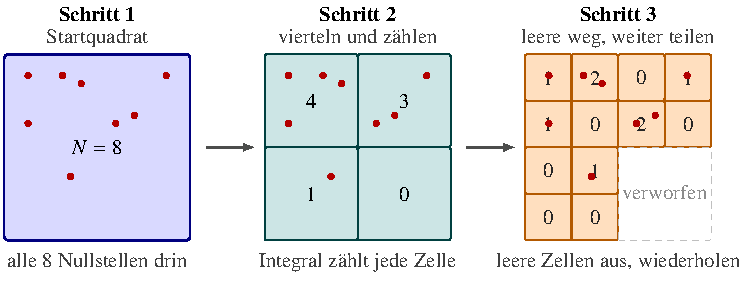
\includegraphics{papers/weyl/images/quadtree.pdf}
\caption{Drei Stadien von Weyls Algorithmus an einem Beispielpolynom mit $8$ Nullstellen.
Links das Startquadrat $D = [-r,r] \times [-r,r]$, das alle Nullstellen umschliesst.
Mitte: nach der ersten Iteration ist $D$ in vier Teilquadrate zerlegt, das
Wegintegral liefert die Nullstellenanzahl jedes Teilquadrats; in unserem Beispiel
$4$, $3$, $1$ und $0$ --- die Probe $4+3+1+0 = 8$ stimmt.
Rechts: das leere Quadrat (unten rechts) wird verworfen, die übrigen drei werden
ihrerseits geviertelt. Der Prozess wiederholt sich, bis jede Nullstelle in einem
eigenen kleinen Quadrat isoliert ist.
\label{weyl:fig:quadtree}}
\end{figure}


\subsection{Abbruch und Übergabe%
\label{weyl:subsection:abbruch}}
Die Iteration läuft so lange, bis jede Nullstelle in einem eigenen Quadrat isoliert
ist, also bis für jedes aktive Quadrat $N(D_i) = 1$ gilt und die Kantenlänge unter eine
vorgegebene Schranke $\varepsilon > 0$ gefallen ist.
An diesem Punkt liefert der Quadtree für jede Nullstelle einen kleinen rechteckigen
Suchbereich, dessen Mittelpunkt eine gute Näherung darstellt.
Die Schranke $\varepsilon$ wählt man nach der gewünschten Genauigkeit.
Soll der Quadtree selbst die Nullstelle bis auf einen Fehler $\eta$ lokalisieren,
nimmt man zum Beispiel $\varepsilon \leq \sqrt{2}\eta$, denn der Mittelpunkt eines
Quadrats der Kantenlänge $\varepsilon$ ist höchstens $\varepsilon/\sqrt{2}$ von
jedem Punkt im Quadrat entfernt.
Wenn der Quadtree nur einen Startwert für das Newton-Verfahren liefern soll, darf
$\varepsilon$ deutlich grösser sein.
In diesem Fall verfeinert man weiter, falls Newton nicht rasch konvergiert oder in
ein anderes Einzugsgebiet zu laufen scheint.

Eine kleine Optimierung ist möglich, sobald für ein aktives Quadrat bereits
$N(D)=1$ bekannt ist, seine Kantenlänge aber noch grösser als $\varepsilon$ ist.
Teilt man dieses Quadrat erneut in vier Kinderquadrate, kann nur eines dieser
Kinder eine Nullstelle enthalten, sofern keine Nullstelle auf einer Teilungslinie
liegt.
Man berechnet die Werte der Kinder dann der Reihe nach und hört auf, sobald ein
Kind mit Wert $1$ gefunden wurde.
Die übrigen Kinder müssen in diesem regulären Fall den Wert $0$ haben und können
verworfen werden.
Findet man kein solches Kind oder treten nichtganzzahlige Werte auf, verwendet man
wieder den vollständigen Selbsttest \eqref{weyl:eq:probe} und verschiebt gegebenenfalls
das Gitter leicht.

Wie viele Iterationen sind nötig?
Die Kantenlänge halbiert sich pro Schritt, die Genauigkeit verdoppelt sich also
pro Runde, genau wie bei der reellen Bisektion.
Um auf $\varepsilon$-Genauigkeit zu kommen, braucht man etwa
$m \approx \log_2(2r/\varepsilon)$ Iterationen.
Für eine Genauigkeit von $10^{-6}$ bei Startradius $r = 10$ sind das rund $24$ Schritte.

\subsection{Pseudocode%
\label{weyl:subsection:pseudocode}}
\index{Pseudocode}%
Stellen wir die Schritte als kompakten Pseudocode zusammen.
Listing~\ref{weyl:alg:quadtree} fasst den Algorithmus zusammen.

\floatname{algorithm}{Algorithmus}

\begin{algorithm}[!h]
\caption{Weyls Quadtree-Algorithmus\label{weyl:alg:quadtree}}
\begin{algorithmic}[1]
\Require Polynom $f$ vom Grad $n$, Genauigkeit $\varepsilon > 0$
\Ensure Liste von Quadraten, die je eine Nullstelle enthalten
\State Wähle Startradius $r$ gemäss \eqref{weyl:eq:startradius}
\State Setze $D_0 \gets [-r,r] \times [-r,r]$
\State $\mathcal{A} \gets \{D_0\}$
  \Comment{Liste aktiver Quadrate}
\State $\mathcal{R} \gets \emptyset$
  \Comment{Liste isolierter Nullstellen}
\While{$\mathcal{A} \neq \emptyset$}
  \State Entnimm ein Quadrat $D$ aus $\mathcal{A}$
  \State Viertle $D$ in $D_1, D_2, D_3, D_4$
  \ForAll{$i = 1, \dots, 4$}
    \State Berechne $N(D_i) = \frac{1}{2\pi i} \oint_{\partial D_i} \frac{f'}{f}\, dz$
    \If{$N(D_i) = 0$}
      \State verwerfe $D_i$
    \ElsIf{$N(D_i) = 1$ und Kantenlänge von $D_i$ $< \varepsilon$}
      \State füge $D_i$ zu $\mathcal{R}$ hinzu
    \Else
      \State füge $D_i$ zu $\mathcal{A}$ hinzu
    \EndIf
  \EndFor
\EndWhile
\State \Return $\mathcal{R}$
\end{algorithmic}
\end{algorithm}

Die einzige nicht-triviale Operation ist die Auswertung des Wegintegrals.
In der hier verwendeten Variante geschieht das numerisch, zum Beispiel mit der
Mittelpunktregel oder mit einem adaptiven Verfahren.
Die Begründung dafür liefert das Argumentprinzip aus der komplexen Analysis
\cite{weyl:eisermann}.
Es gibt auch algebraische Varianten.
Dabei führt man die Zählung mit euklidischer Polynomdivision auf Sturm-Folgen
beziehungsweise Cauchy-Indizes zurück \cite{weyl:stoer-bulirsch}.
Da der Integrand $f'/f$ rational ist und das Resultat eine ganze Zahl sein muss, genügt
schon eine moderate numerische Genauigkeit. Ein Fehler kleiner als $\tfrac{1}{2}$
identifiziert die korrekte ganze Zahl eindeutig.

\subsection{Ein durchgerechnetes Beispiel%
\label{weyl:subsection:beispiel}}
Wir illustrieren den Algorithmus am Polynom
\begin{equation}
f(z)
=
z^3 - 2z + 2
,
\label{weyl:eq:beispiel-polynom}
\end{equation}
mit Ableitung $f'(z) = 3z^2 - 2$.
Die exakten Nullstellen lassen sich noch mit der Formel von Cardano berechnen und
\index{Cardano, Gerolamo}%
lauten näherungsweise
\[
\alpha_1 \approx -1.7693
,
\qquad
\alpha_{2,3} \approx 0.8846 \pm 0.5897\,i
.
\]
Wir tun aber so, als kennen wir sie nicht, und lassen den Algorithmus arbeiten.
Als Genauigkeit wählen wir in diesem Beispiel $\varepsilon = 10^{-6}$.
Mit dem Startradius $r=4$ wären nach der Abschätzung
$m \approx \log_2(2r/\varepsilon)$ rund $23$ Quadtree-Verfeinerungen nötig, um alle
Nullstellen allein durch den Quadtree bis auf diese Kantenlänge zu lokalisieren.
Für die Kombination mit Newton werden wir jedoch deutlich früher übergeben.

\subsubsection*{Startquadrat}
Mit den Koeffizienten $a_0 = 2$, $a_1 = -2$, $a_2 = 0$, $a_3 = 1$ liefert die Formel
\eqref{weyl:eq:startradius}
\[
\max
\left\{
\sqrt[3]{4\cdot 2},
\sqrt{4\cdot 2},
0
\right\}
=
\sqrt{8}
<
3
,
\]
also wäre bereits $r=3$ zulässig.
Wir wählen für das Beispiel den etwas grösseren Radius $r=4$ und damit
$D_0 = [-4, 4] \times [-4, 4]$ als Startquadrat.
Die numerische Auswertung von $N(D_0)$ mittels Mittelpunktregel auf jeder Seite
ergibt den Wert $3$, in Übereinstimmung
mit dem Grad des Polynoms.

\subsubsection*{Erste Iteration}
Vierteln von $D_0$ liefert die vier Teilquadrate
\begin{align*}
D_1 &= [-4, 0] \times [0, 4],
&
D_2 &= [0, 4] \times [0, 4],
\\
D_3 &= [-4, 0] \times [-4, 0],
&
D_4 &= [0, 4] \times [-4, 0].
\end{align*}
Die Auswertung der Wegintegrale liefert allerdings nicht ganzzahlige Werte:
$N(D_1) \approx 0.5 - 1.01\,i$ und $N(D_3) \approx 0.5 + 1.01\,i$.
Das ist kein Rechenfehler, sondern die Symptomatik des in
Abschnitt~\ref{weyl:subsection:mehrfache} angesprochenen Sonderfalls. Die reelle
Nullstelle $\alpha_1 \approx -1.7693$ liegt exakt auf dem Rand $y = 0$ zwischen $D_1$
und $D_3$.
Wir verschieben das Gitter um einen kleinen Betrag $\delta = 10^{-2}$ und teilen
stattdessen bei der waagerechten Linie $y = \delta$.
Mit dieser Korrektur ergibt die erste Iteration
\begin{center}
\begin{tabular}{lc}
\toprule
Teilquadrat & $N$ \\
\midrule
$D_1' = [-4, 0] \times [\delta, 4]$ & $0$ \\
$D_2' = [0, 4] \times [\delta, 4]$ & $1$ \\
$D_3' = [-4, 0] \times [-4, \delta]$ & $1$ \\
$D_4' = [0, 4] \times [-4, \delta]$ & $1$ \\
\midrule
Summe & $3$ \\
\bottomrule
\end{tabular}
\end{center}
Die Probe stimmt, und $D_1'$ wird als nullstellenfrei verworfen.
Schon nach einer Iteration sind die drei Nullstellen voneinander getrennt.

\subsubsection*{Weitere Iterationen}
Wir konzentrieren uns auf $D_2'$, das die Nullstelle $\alpha_2 \approx 0.8846 + 0.5897\,i$
enthält.
Vierteln liefert vier Teilquadrate, von denen drei leer sind und nur das
Quadrat $[0, 2] \times [\delta, 2.005]$ den Wert $N = 1$ liefert.
Eine weitere Vierteln-Runde isoliert die Nullstelle im Quadrat
$[0, 1] \times [\delta, 1.008]$ mit Kantenlänge $\approx 1$.
Würde man ausschliesslich den Quadtree verwenden, müsste man nun bis zur Kantenlänge
$\varepsilon = 10^{-6}$ weiterteilen.
Für die Hybrid-Variante übergeben wir stattdessen schon nach wenigen Schritten den
Mittelpunkt an das Newton-Verfahren.

\subsubsection*{Übergabe an Newton}
Brechen wir bereits nach der ersten Vierteln-Runde innerhalb von $D_2'$ ab und
nehmen den groben Mittelpunkt $\hat z = 1 + i$ als Startwert für die Newton-Iteration
\[
z_{k+1}
=
z_k
-
\frac{z_k^3 - 2 z_k + 2}{3 z_k^2 - 2}
,
\]
Dabei bezeichnet $z_k$ den $k$-ten Newton-Iterierten; die Zielnullstelle ist
$\alpha_2$.
Damit erhalten wir die folgende Tabelle, in der die Anfangsziffern unterstrichen sind,
die bereits mit der Zielnullstelle übereinstimmen.
\begin{center}
\begin{tabular}{>{$}r<{$}>{$}l<{$}>{$}r<{$}}
\toprule
k & z_k                                                                        & |z_k - \alpha_2|\phantom{0}  \\
\midrule
0 & 1.0000\phantom{000000} + 1.0000\,i\phantom{000000}                         & 4.3 \cdot 10^{-1\phantom{0}} \\
1 & 0.9000\phantom{000000} + 0.7000\,i\phantom{000000}                         & 1.1 \cdot 10^{-1\phantom{0}} \\
2 & 0.\underline{88}37\phantom{000000} + 0.6003\,i\phantom{000000}             & 1.1 \cdot 10^{-2\phantom{0}} \\
3 & 0.\underline{8846}\phantom{000000} + 0.\underline{589}8\,i\phantom{000000} & 1.1 \cdot 10^{-4\phantom{0}} \\
4 & 0.\underline{8846461}653 + 0.\underline{58974280}62\,i                     & 1.2 \cdot 10^{-8\phantom{0}} \\
5 & 0.\underline{8846461771} + 0.\underline{5897428050}\,i                     & < 10^{-10}                   \\
\bottomrule
\end{tabular}
\end{center}
Die quadratische Konvergenz ist gut zu erkennen. Die Anzahl korrekter Nachkommastellen
verdoppelt sich von Schritt zu Schritt und nach fünf Iterationen ist die
Maschinengenauigkeit nahezu erreicht.
Zugleich bleiben alle aufgeführten Iterierten im übergebenen Quadrat
$[0, 2] \times [\delta, 2.005]$.
Das ist ein einfacher nachträglicher Test dafür, dass das Quadrat für die Übergabe
an Newton klein genug gewählt wurde.
Für $\alpha_3 = \overline{\alpha_2}$ und $\alpha_1$ verläuft das Verfahren analog mit jeweils
eigenem Startquadrat.

Dieses kleine Beispiel illustriert die Hauptpunkte des Algorithmus auf engem Raum.
Die Probe \eqref{weyl:eq:probe} fängt einen Rand-Sonderfall ab, der Quadtree trennt
die drei Nullstellen schon innerhalb weniger Iterationen und das Newton-Verfahren
übernimmt für die Feinkonvergenz die letzten Dezimalstellen in wenigen Schritten.

\subsection{Mehrfache Nullstellen und Sonderfälle%
\label{weyl:subsection:mehrfache}}
Liegen mehrere Nullstellen sehr nah beieinander oder fällt eine mehrfache Nullstelle
in ein Quadrat, so bleibt $N(D_i) \geq 2$, auch wenn das Quadrat schon klein ist.
Der Algorithmus erkennt das automatisch und teilt weiter, bis sich die Nullstellen
trennen oder das Quadrat so klein wird, dass man die Nullstellen als praktisch
zusammenfallend betrachten kann.
\index{Nullstelle!mehrfache}%
Liegt eine echte mehrfache Nullstelle vor, terminiert das Verfahren erst wenn die
Kantenlänge unter $\varepsilon$ fällt. Das Quadrat mit $N(D_i) = k > 1$ wird dann mit
dem Hinweis {$k$-fache Nullstelle} ausgegeben.
Das gewöhnliche Newton-Verfahren hilft in diesem Fall nicht im gleichen Mass wie
bei einfachen Nullstellen. An einer mehrfachen Nullstelle verschwindet auch die
Ableitung, und die quadratische Konvergenz geht verloren. Selbst bei einem guten
\index{Konvergenz!linear}%
Startwert konvergiert die Newton-Iteration dann im Allgemeinen nur linear. Deshalb
bleibt die Bisektion bis zur vorgeschriebenen Genauigkeit die robuste Variante.
Ein modifiziertes Newton-Verfahren wäre erst dann naheliegend, wenn die
Vielfachheit der Nullstelle bereits bekannt ist.

Liegt zufällig eine Nullstelle exakt auf dem Rand $\partial D_i$ eines Quadrats, so ist
das Integral nicht wohldefiniert.
In der Praxis verschiebt man dann die Gitterlinien um einen kleinen Betrag oder
verwendet ein leicht verschobenes Startquadrat. Da es nur endlich viele Nullstellen
gibt, lässt sich diese Situation immer vermeiden.
